\begin{figure}[H]
    \centering
    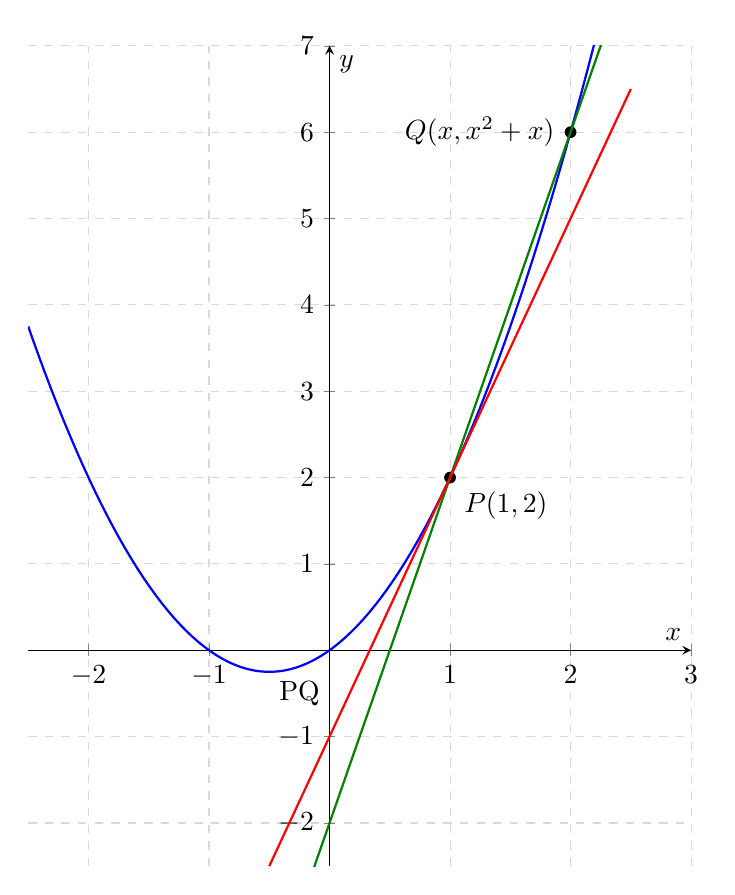
\begin{tikzpicture}
        \begin{axis}[
            axis lines=middle,
            xlabel=$x$,
            ylabel=$y$,
            xmin=-2.5, xmax=3,
            ymin=-2.5, ymax=7,
            legend pos=north west,
            grid=major,
            grid style={dashed, gray!30},
            width=10cm,
            height=12cm,
        ]
        
        % Đồ thị Parabol
        \addplot[domain=-2.5:2.5, samples=100, thick, blue, legend entries={$y=x^2+x$}] {x^2+x};
        
        % Điểm P và Q
        \node[circle, fill, inner sep=1.5pt, label={below right:$P(1,2)$}] at (axis cs:1,2) {};
        \node[circle, fill, inner sep=1.5pt, label={left:$Q(x, x^2+x)$}] at (axis cs:2,6) {};
        
        % Cát tuyến PQ
        \addplot[domain=-0.5:2.5, thick, green!50!black] {4*x-2};
        \node at (axis cs:0,-0.25) [anchor=north east] {PQ};

        % Tiếp tuyến t
        \addplot[domain=-0.5:2.5, thick, red, legend entries={$t$}] {3*x-1};
        
        \end{axis}
    \end{tikzpicture}
    \caption{Cát tuyến $PQ$ tiến dần về tiếp tuyến $t$ khi $Q \to P$.}
    \label{fig:tangent_of_parabola}
\end{figure}